\section{Timing Compartments}
Timing compartments are a new architecture primitive that control timing 
channel leakage among software entities that share hardware. When combined with 
explicit channel protection (such as access controls) timing compartments 
provide total software isolation.
A timing compartment conatins one or more software entities. Here, a software 
entitiy is some system abstraction (such as processes or threads in a single OS 
system or virtual machines in a virtualization based system) that execute 
software and have an owner. Intuitively, a single timing compartment contains 
only software entities that trust each other explicitly (such as all the VMs on 
a machine owned by the same user) or implicitly (all the VMs that do not want 
to pay for protection), and leakage within a timing compartment is safe.

Timing channels between timing compartments must be controlled according to a 
policy that meets the security requirements of the system. This policy entails 
of a lattice of security levels such as $\mathtt{low} \leq
\mathtt{high}$. A timing compartment can only leak information to a preceeding 
timing compartment in the lattice. This lattice model is quite expressive. The 
lattice $\mathtt{low} \leq \mathtt{high}$ defines a policy where a high 
assurance software entitycan not leak information to a low assurance one. The 
lattice $\mathtt{T_1} \nleq \mathtt{T_2}, \mathtt{T_2} \nleq \mathtt{T_1}$ 
defines a policy where $T_1$ and $T_2$ are mutually distrusting. By convention, 
security lables share names with their timing compartments. 

To enforce the policy, a trusted software component called the timing 
compartment manager (TCM) confines software entities into TCs. The TCM then 
informs the hardware of the TCs and policy. At runtime, the TCM tags software 
requests for hardware to indicate the TC of the software entity that made the 
request. The hardware then enforces the policy by controlling how requests from 
different TCs share resources.

Timing compartments only address timing channels; they do not control 
information flow through explicit channels. Handling these concerns separately 
allows for more flexibility in the overall system design.  When designing a 
secure system, implementors must consider how the cost required to carry out a 
particular attack compares with other attacks, the potential damage that could 
be caused by an attack, and the cost and performance impact of implementing the 
security mechanisms needed to stop it. This enables timing compartments to 
provide timing channel protection only to software entities that need it.

\subsection{Applications}
This section describes several application domains and vulnerable systems that 
conform to our threat model. We show how each can be protected with timing 
compartments.
\subsubsection{Cloud Computing}
In platform as a service cloud computing, a cloud provider owns hardware which 
is shared by virtual machines that are managed by a hypervisor. The cloud 
provider leases out virtual machines to clients. However, tenants in a cloud 
computing environment have no control over the VMs they co-reside with; they 
may share hardware with competitors or attackers that want to extract sensitive
data. One purpose of machine virtualization is to isolate separate OS 
environments, but the platform as a whole is still less secure than executing 
on separate hardware. Timing channels can violate VM isolation. For some 
clients without strong security requirements, this is not a concern, but for 
others, this security threat makes cloud computing inviable.

Figure \ref{fig:cloud_tcs} shows an example cloud computing environment with 
four virtual machines that have different security requirements. Each VM in the 
system implicitly trusts the hypervisor. VM1 and VM2 are running programs with 
high security requirements. VM1 and VM2 are mutually distrusting and distrust 
all other VMs in the environment.  VM3 and VM4 run an applications that have 
low security requirements, but are very performance intensive. VM3 and VM4 
still need the explicit channel isolation provided by machine virtualization, 
but the owners would rather not incur performance overheads for unneeded timing 
channel protection.

\begin{figure}
    \begin{center}
        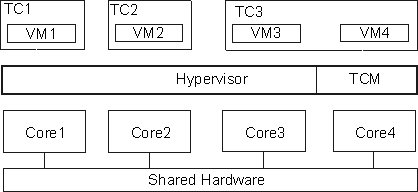
\includegraphics[width=1.51in]{figs/cloud_tcs.pdf}
        \caption{A cloud environment with timing channel vulnerabilites.  VM1 
        and VM2 have high security requirements, but VM3 and VM4 do not.}
        \label{fig:cloud_tcs}
    \end{center}
\end{figure}

Figure \ref{fig:cloud_tcs} shows how timing compartments can be applied to meet 
the needs of this system. VM1 and VM2 are confined to their own timing 
compartments TC1 and TC2, but VM3 and VM4 are grouped in TC3.  The lattice $TC3 
\leq TC1, TC3 \leq TC2, TC1 \nleq T2, TC2 \nleq TC1$ specifies the policy. TC3 
preceeds both TC1 and TC2 implying timing channel leakage from VM3 or VM4 to 
any other VM is not controlled. However, VM1 and VM2 cannot leak information to 
VM3 or VM4. Additionally, VM1 and VM2 cannot leak information to each other 
since TC1 and TC2 are incomparable. This meets the security requirements of VM1 
and VM2 since both are totally isolated from the other VMs through timing 
channels. Since VM3 and VM4 share a timing compartment, they can share 
resources normally and incur minimal performance overheads.
